\documentclass[12pt]{article}

% ------------------------------------------------------------
% Page Layout
% ------------------------------------------------------------

\usepackage{geometry}
\geometry{margin=1in}

\usepackage{setspace}
\onehalfspacing

% ------------------------------------------------------------
% Mathematics
% ------------------------------------------------------------

\usepackage{amsmath}
\usepackage{amssymb}
\usepackage{mathtools}
\usepackage{amsthm}

% ------------------------------------------------------------
% Diagrams
% ------------------------------------------------------------

\usepackage{tikz}
\usepackage{tikz-cd}
\usetikzlibrary{positioning,shapes.geometric,arrows.meta}

% ------------------------------------------------------------
% Hyperlinks
% ------------------------------------------------------------

\usepackage{hyperref}
\hypersetup{
  colorlinks=true,
  linkcolor=black,
  citecolor=black,
  urlcolor=blue
}

% ------------------------------------------------------------
% Theorem Environments
% ------------------------------------------------------------

\newtheorem{definition}{Definition}[section]
\newtheorem{theorem}{Theorem}[section]
\newtheorem{proposition}{Proposition}[section]
\newtheorem{corollary}{Corollary}[section]
\newtheorem{remark}{Remark}[section]
\newtheorem{example}{Example}[section]

% ------------------------------------------------------------
% Spherepop Operator Macros
% ------------------------------------------------------------

\newcommand{\Pop}{\operatorname{\textsc{Pop}}}
\newcommand{\Bind}{\operatorname{\textsc{Bind}}}
\newcommand{\Collapse}{\operatorname{\textsc{Collapse}}}

\newcommand{\History}{\mathcal{H}}
\newcommand{\Option}{\Omega}
\newcommand{\State}{\mathcal{S}}
\newcommand{\Seq}[1]{\left[#1\right]}
\newcommand{\Append}{\mathbin{\cdot}}

% ------------------------------------------------------------
% Title
% ------------------------------------------------------------

\title{History as Identity:\\
The Append-Only Algebra of Spherepop}

\author{Flyxion}

\date{\today}

% ------------------------------------------------------------
% Document
% ------------------------------------------------------------

\begin{document}

\maketitle

% ============================================================
\begin{abstract}
% ============================================================

Many computational models identify a process with its observable
input-output behavior and discard the internal sequence of
operations that produced that behavior. In systems governed by
irreversible commitments, however, this internal sequence often
carries essential information about causality and provenance.

This paper introduces \emph{Spherepop}, a minimal algebraic
framework in which the identity of a computation is its
append-only history of commitments rather than its final state.
A Spherepop state is represented by a residual option space
together with an accumulated commitment history. Three primitive
operators---$\Pop$, $\Bind$, and $\Collapse$---govern the
evolution of this structure: $\Pop$ records irreversible
commitments, $\Bind$ restricts admissible options without
committing, and $\Collapse$ reconstructs observable state from
the resulting history.

We show that these operators generate a free history category
whose morphisms are ordered commitment sequences, prove that the
operator set is minimal, and establish that conventional state
semantics arises as a quotient of this structure obtained by
identifying histories with identical observable outcomes.
This perspective clarifies the structure of systems whose natural
representation is append-only, including event-sourced
architectures, version control systems, and causal process models.

\end{abstract}

\newpage
\tableofcontents
\newpage

% ============================================================
\section{Introduction}
% ============================================================

A recurring ambition in the theory of computation is the identification of the minimal mathematical structure required to model a class of phenomena faithfully. For deterministic sequential computation that structure is the Turing machine or equivalently the $\lambda$-calculus; for concurrent interaction it is process algebra or the $\pi$-calculus; for feedback and recursion within monoidal categories it is the traced monoidal category of Joyal, Street, and Verity. In each case the theory achieves its power by deciding what to abstract over and what to preserve.

Traces, in particular, achieve their power precisely by abstraction. The trace operator $\mathrm{Tr}^U_{A,B}(f)$ for a morphism $f : A \otimes U \to B \otimes U$ asserts that the precise internal behavior on the ``feedback wire'' $U$ is irrelevant once its effect on the external interface $A \to B$ is determined. The loop is collapsed; what remains is the fixed-point input-output relation.

Spherepop originates from the refusal of precisely this identification. Its central commitment is that the internal path---the ordered sequence of decisions, exclusions, and contextual restrictions that produced an observable state---is not auxiliary information to be discarded once a result is known. It is the result. Two computations that terminate at the same value but follow different causal chains are, in Spherepop's ontology, distinct objects. The identity of a process is its history, not its output.

\subsection{Contributions}

The aim of this paper is to formalize the intuition that, in many
systems governed by irreversible commitments, the identity of a
process is determined by the ordered history of those commitments
rather than by its final state alone. The principal contributions
are threefold.

First, we introduce a minimal state representation consisting of a residual option space and an append-only commitment history, capturing the distinction between possibilities that remain available and decisions that have already been made.

Second, we define three primitive operators---$\Pop$, $\Bind$, and $\Collapse$---prove that they constitute a minimal generating set for the history algebra, and establish their principal algebraic properties including monotonicity, non-commutativity, and functoriality of collapse.

Third, we characterize the resulting structure categorically as a free history category and demonstrate that conventional state semantics arises as a quotient of this richer history-based representation. In this formulation observable states appear as compressed summaries of the commitment histories that generated them, and the collapse functor is shown to be left adjoint to the history embedding.

Together these results provide a compact mathematical framework for systems whose natural semantics is append-only and history-preserving, including event-sourced architectures, version control systems, causal process models, and many forms of practical decision making.

\subsection{Outline}

This essay develops the formal structure underlying these contributions and accompanies each stage of the formalism with intuitive analogies. Section~\ref{sec:related} situates the work relative to existing literature. Section~\ref{sec:notation} establishes notation. Section~\ref{sec:intuition} presents the central idea in ordinary language. Section~\ref{sec:traces} reviews traced monoidal categories and isolates precisely what the trace operator discards. Section~\ref{sec:state} introduces the Spherepop state representation. Section~\ref{sec:operators} defines the three primitive operators. Section~\ref{sec:properties} establishes their algebraic properties. Section~\ref{sec:minimality} proves minimality of the operator set. Section~\ref{sec:example} works through a minimal example. Section~\ref{sec:deterministic} establishes the representation theorem for deterministic computation. Section~\ref{sec:quotient} characterizes state semantics as a quotient of history semantics. Section~\ref{sec:algebra} describes the history algebra. Section~\ref{sec:historycategory} gives the categorical treatment. Section~\ref{sec:adjunction} establishes the collapse-history adjunction. Sections~\ref{sec:partialorders} through~\ref{sec:cognition} draw connections to concurrency, entropy, programming practice, and reasoning. Section~\ref{sec:limitations} discusses limitations. Section~\ref{sec:conclusion} draws the principal conclusions.

% ============================================================
\section{Related Work}
\label{sec:related}
% ============================================================

The Spherepop framework intersects several existing research traditions concerned with the structure of computation, causality, and state evolution.

\paragraph{Categorical semantics of computation.} Category theory has long provided a language for describing the structure of computational processes. The traced monoidal categories introduced by Joyal, Street, and Verity \cite{joyal1996} give a categorical account of feedback and recursion in monoidal settings. In traced semantics internal loops may be collapsed into morphisms representing the overall input-output behavior of a system. Spherepop differs from traced semantics in its treatment of internal computation: rather than identifying morphisms that exhibit the same external behavior, the framework developed here preserves the ordered sequence of commitments that produced the result. Traced semantics may therefore be understood as a quotient of the richer history structure considered in this paper.

\paragraph{Concurrency and event structures.} The study of concurrent computation has produced several models in which system behavior is represented by partially ordered events rather than sequential state transitions \cite{winskel1995}. The generalization of Spherepop histories to partially ordered structures, discussed in Section~\ref{sec:partialorders}, places the framework in close conceptual proximity to these models.

\paragraph{Distributed systems and append-only logs.} Event-sourced architectures \cite{fowler2005} reconstruct state by replaying a sequence of recorded events, while distributed databases often maintain conflict-free replicated data types whose histories converge through causal merging \cite{shapiro2011}. Version control systems such as Git record software evolution as a directed acyclic graph of commits \cite{chacon2014}. These systems share a structural property central to Spherepop: the observable state is derived from a history of irreversible events.

\paragraph{Causal models in physics.} Causal set theory models spacetime as a partially ordered set of events whose order encodes causal precedence \cite{brightwell1991}. Although the present work is concerned with computational semantics rather than physical ontology, the structural similarity highlights the generality of history-based descriptions.

\paragraph{Position of the present work.} The contribution of this paper is to isolate a minimal algebraic framework that captures the append-only structure common to these domains. By introducing a simple state representation and three primitive operators, the framework provides a compact language for describing processes whose identity is determined by the ordered history of commitments through which they evolve.

% ============================================================
\section{Notation and Conventions}
\label{sec:notation}
% ============================================================

This section summarizes the principal symbols and conventions used throughout the paper.

The symbol $\Option$ denotes a finite \emph{option space} whose elements represent the possible commitments available to a Spherepop process. At time $t$ the set of admissible possibilities is written $\Option_t \subseteq \Option$ and is called the \emph{residual option space}.

Commitment histories are finite ordered sequences of elements of $\Option$. A history is written $H = \Seq{x_1,\dots,x_n}$ where $x_i \in \Option$ represents the $i$th commitment. The empty history is denoted $\varnothing$. When two histories are concatenated we write $H_1 \Append H_2$.

The three primitive operators are written $\Pop$, $\Bind$, and $\Collapse$. The operator $\Pop_x$ represents an irreversible commitment to element $x \in \Option_t$. The operator $\Bind_f$ represents a contextual restriction by an admissibility function $f$. The operator $\Collapse$ reconstructs observable state from the commitment history.

Observable states belong to a category $\State$ of states and state transformations. The collapse operation induces a functor $\Collapse : \History(\Option) \to \State$ from the free history category to the category of observable states. All option spaces are assumed finite unless otherwise stated.

% ============================================================
\section{Why Histories Matter: The Central Idea}
\label{sec:intuition}
% ============================================================

Before turning to the formal mathematics it is useful to state the central idea of Spherepop in ordinary language and to give the reader a collection of concrete images to hold in mind while the formalism is developed.

\subsection{Programs as Functions vs.\ Programs as Histories}

Most computational models treat a program as a function. You provide an input, the program runs, and eventually it produces an output. Once the output is known, the intermediate steps that produced it are usually discarded. They were merely a means to an end.

Spherepop treats those intermediate steps differently. Instead of discarding them, it records them permanently. The sequence of steps becomes the primary object of study.

The same contrast appears outside computing. If you edit a document repeatedly and keep only the final version, the intermediate drafts disappear. If instead you use a version control system, every change is recorded in a commit log. The identity of the document is no longer just the final text; it is the entire sequence of edits that produced it. Spherepop adopts the second perspective.

\subsection{The Restaurant Analogy}

Another illustration comes from everyday decision making. Imagine choosing a restaurant for dinner. The final choice may be ``Italian.'' But the path to that choice matters. Perhaps Mexican was ruled out because the restaurant was closed, and sushi was ruled out because a friend dislikes it. Two evenings may end at the same restaurant yet involve entirely different chains of reasoning. In Spherepop those chains are preserved: what was eliminated, in what order, and by what constraint.

\subsection{The Bubble Analogy}

A visual way to picture the Spherepop state is to imagine a row of labeled bubbles floating in front of you. Each bubble represents a possible choice. As the computation proceeds, bubbles are popped one at a time. A popped bubble cannot be restored. The row of remaining bubbles shrinks, while the sequence of popped bubbles grows and is preserved as the record of what happened. The name ``Spherepop'' comes from this image.

\subsection{Visual Summary of the Two Perspectives}

The following two diagrams contrast the trace perspective with the Spherepop perspective.

\begin{figure}[h]
\centering
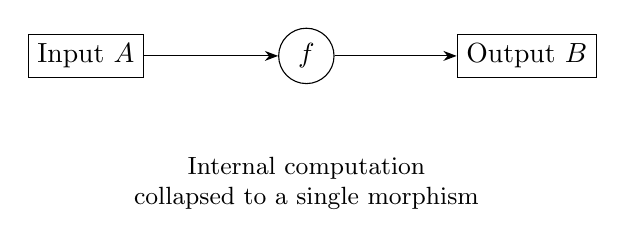
\begin{tikzpicture}[>=Stealth,node distance=2.8cm]
\node[draw,rectangle] (A) {Input $A$};
\node[draw,circle,right of=A] (f) {$f$};
\node[draw,rectangle,right of=f] (B) {Output $B$};
\draw[->] (A) -- (f);
\draw[->] (f) -- (B);
\node[below=0.8cm of f,align=center,font=\small]
  {Internal computation\\collapsed to a single morphism};
\end{tikzpicture}
\caption{Trace-style semantics. Internal computation is abstracted away
and represented only by its overall input-output behavior.}
\end{figure}

\begin{figure}[h]
\centering
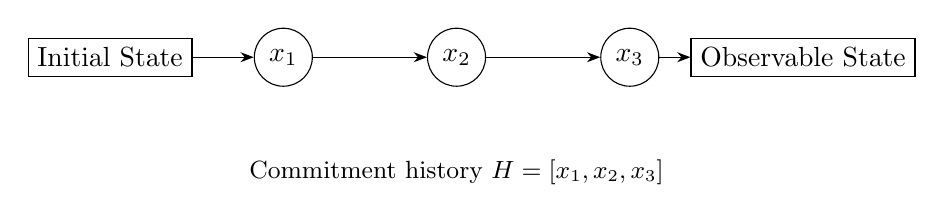
\begin{tikzpicture}[>=Stealth,node distance=2.2cm]
\node[draw,rectangle] (s0) {Initial State};
\node[draw,circle,right of=s0] (x1) {$x_1$};
\node[draw,circle,right of=x1] (x2) {$x_2$};
\node[draw,circle,right of=x2] (x3) {$x_3$};
\node[draw,rectangle,right of=x3] (s) {Observable State};
\draw[->] (s0) -- (x1);
\draw[->] (x1) -- (x2);
\draw[->] (x2) -- (x3);
\draw[->] (x3) -- (s);
\node[below=0.8cm of x2,align=center,font=\small]
  {Commitment history $H = \Seq{x_1,x_2,x_3}$};
\end{tikzpicture}
\caption{Spherepop semantics. The computation is represented by the
ordered history of commitments that produced the observable state.}
\end{figure}

% ============================================================
\section{The Trace Operator and What It Hides}
\label{sec:traces}
% ============================================================

Before examining what Spherepop preserves, it is useful to be precise about what the trace operator discards.

\subsection{What the Trace Does}

The trace can be understood informally as a formal way of saying that the internal workings of a system are irrelevant once its external behavior is known. Trace semantics allows the program to contain internal loops, recursive calls, and intermediate computations, yet collapses all of those details into a single morphism $f : A \to B$.

\medskip\noindent\textbf{Film analogy.} Imagine watching a film and then writing a one-sentence plot summary. The summary may capture the overall outcome of the story but does not contain the sequence of scenes that produced it. Trace semantics treats the program like the summary. Spherepop treats it like the full film.\medskip

\begin{definition}[Traced monoidal category]
A \emph{traced symmetric monoidal category} is a symmetric monoidal category $(\mathcal{C}, \otimes, I)$ equipped with a family of functions
\[
\mathrm{Tr}^U_{A,B} : \mathcal{C}(A \otimes U,\, B \otimes U) \;\longrightarrow\; \mathcal{C}(A, B),
\]
one for each triple of objects $A, B, U$, satisfying naturality, dinaturality, vanishing, and the yanking equation $\mathrm{Tr}^U_{U,U}(\sigma_{U,U}) = \mathrm{id}_U$.
\end{definition}

The dinaturality condition ensures that the trace is insensitive to the choice of representation for the internal computation: any two morphisms related by an internal change of type produce equal traces.

\subsection{What the Trace Forgets}

The trace performs a specific act of forgetting. It discards the ordered chain of intermediate steps that produced the output. Two programs that produce the same external function are identified as the same morphism regardless of their internal histories. In categorical language, trace semantics constructs a quotient that identifies morphisms whose internal behavior differs but whose external effect is the same. Spherepop declines that quotient and preserves the histories themselves.

\begin{remark}
Consider two recursive programs that both compute the identity function $A \to A$. One returns immediately; the other performs a thousand recursive calls that cancel before returning. Under traced monoidal semantics both programs denote the same morphism $\mathrm{id}_A$. Under Spherepop semantics the programs differ because the commitment histories differ.
\end{remark}

% ============================================================
\section{State Representation: Option Space and History}
\label{sec:state}
% ============================================================

The primitive data structure of Spherepop is a pair representing the current state of an unfolding process.

\begin{definition}[Spherepop state]
\label{def:state}
Let $\Option$ be a finite set called the \emph{option space}. A \emph{Spherepop state} is a pair
\[
(\Option_t,\, H_t)
\]
where $\Option_t \subseteq \Option$ is the \emph{residual option space} at time $t$ and $H_t = \Seq{x_1, x_2, \ldots, x_k}$ is the \emph{commitment history}, an ordered list of elements that have been selected and recorded.
\end{definition}

The initial state is $(\Option, \varnothing)$. As the computation proceeds, $\Option_t$ shrinks monotonically and $H_t$ grows monotonically. These two monotonicity conditions are the central structural constraints of the framework.

The option space $\Option_t$ records what \emph{could have happened but did not}; the history $H_t$ records what \emph{did happen}. The asymmetry between them is intentional: the future is an unordered cloud of possibilities while the past is an ordered causal chain.

\begin{example}
Let $\Option = \{a, b, c\}$. After committing to $a$ the state becomes $(\{b,c\},\, \Seq{a})$. After committing to $b$ it becomes $(\{c\},\, \Seq{a,b})$. An alternative computation might produce $(\{c\},\, \Seq{b,a})$. Both states share the same residual option space, but their histories are distinct ordered lists. In Spherepop these are distinct processes.
\end{example}

% ============================================================
\section{The Three Primitive Operators}
\label{sec:operators}
% ============================================================

Three operators act on Spherepop states and constitute the complete operational vocabulary of the framework.

\subsection{Pop: Irreversible Commitment}

\medskip\noindent\textbf{The bubble image.} $\Pop$ is the act of popping one of the floating bubbles. The bubble disappears from the row and its label is appended to the record. The action cannot be undone.\medskip

\begin{definition}[$\Pop$]
Let $(\Option_t, H_t)$ be a Spherepop state and let $x \in \Option_t$. The operator $\Pop_x$ acts as
\[
\Pop_x(\Option_t,\, H_t) \;=\; \bigl(\Option_t \setminus \{x\},\;\; H_t \Append x\bigr).
\]
\end{definition}

The element $x$ is removed from $\Option_t$ and appended to $H_t$ simultaneously. The operation is irreversible: there is no $\Pop^{-1}$ that restores $x$ to the option space and removes it from the history.

\subsection{Bind: Contextual Restriction}

\medskip\noindent\textbf{The menu analogy.} Before choosing a dish you filter the menu by dietary restriction. This filtering removes options without constituting a choice. $\Bind$ is that filter. Eliminated options leave no trace in the decision history because they were never genuine candidates.\medskip

\begin{definition}[$\Bind$]
Let $f : 2^\Option \to 2^\Option$ satisfy $f(\Option_t) \subseteq \Option_t$ for all $\Option_t$. The operator $\Bind_f$ acts as
\[
\Bind_f(\Option_t,\, H_t) \;=\; \bigl(f(\Option_t),\;\; H_t\bigr).
\]
\end{definition}

The history is unchanged because no commitment has occurred. Elements in $\Option_t \setminus f(\Option_t)$ are silently excluded. The distinction between exclusion by $\Bind$ and exclusion by $\Pop$ encodes the difference between structural impossibility and chosen commitment.

\subsection{Collapse: Reconstruction from History}

\medskip\noindent\textbf{The ledger analogy.} A bank account stores a ledger of deposits and withdrawals rather than a fixed balance. The current balance is computed by replaying the ledger. $\Collapse$ is that replay operation.\medskip

\begin{definition}[$\Collapse$]
Let $s_0$ be a fixed root state and let $\{T_x\}_{x \in \Option}$ be a family of state transformations. For a history $H_t = \Seq{x_1, x_2, \ldots, x_n}$, the operator $\Collapse$ acts as
\[
\Collapse(H_t) \;=\; T_{x_n} \circ T_{x_{n-1}} \circ \cdots \circ T_{x_1}(s_0).
\]
\end{definition}

The observable state is derived by composing transformations in temporal order. In general $T_a \circ T_b \neq T_b \circ T_a$, so histories $\Seq{a,b}$ and $\Seq{b,a}$ may yield different observable states. The history must therefore be an ordered list rather than a set.

% ============================================================
\section{Algebraic Properties of the Spherepop Operators}
\label{sec:properties}
% ============================================================

The operators exhibit several structural properties that follow directly from the monotonic nature of commitment histories.

\begin{proposition}[Monotonicity of option spaces]
Let $(\Option_t,H_t)$ be a Spherepop state. After any sequence of operations the option space satisfies $\Option_{t+1} \subseteq \Option_t$.
\end{proposition}

\begin{proof}
Both $\Pop$ and $\Bind$ replace $\Option_t$ with a subset of itself: $\Pop_x$ removes one element, while $\Bind_f$ replaces $\Option_t$ with $f(\Option_t) \subseteq \Option_t$ by definition.
\end{proof}

\begin{proposition}[History extension]
For every Spherepop computation the commitment history satisfies $H_t \preceq H_{t+1}$, where $\preceq$ denotes the prefix relation on sequences.
\end{proposition}

\begin{proof}
$\Bind$ leaves the history unchanged, while $\Pop$ appends one element. In either case $H_{t+1}$ contains $H_t$ as a prefix.
\end{proof}

\begin{proposition}[Non-commutativity of commitments]
For $a,b \in \Option$ with $a \neq b$, in general $\Pop_a \circ \Pop_b \neq \Pop_b \circ \Pop_a$.
\end{proposition}

\begin{proof}
$\Pop_a$ followed by $\Pop_b$ produces history $\Seq{a,b}$, while the reverse order produces $\Seq{b,a}$. Since histories are ordered lists these sequences are distinct whenever $a \neq b$.
\end{proof}

Non-commutativity is essential: if commitments commuted, the causal ordering of events would disappear from the model.

\begin{proposition}[$\Collapse$ as a functor]
The operator $\Collapse$ defines a functor from the free history category $\History(\Option)$ to the category of observable states.
\end{proposition}

\begin{proof}
For histories $H_1$ and $H_2$, $\Collapse(H_1 \Append H_2) = \Collapse(H_2) \circ \Collapse(H_1)$. Concatenation of histories therefore corresponds to composition of state transformations. Identity histories map to identity transformations, establishing functoriality.
\end{proof}

% ============================================================
\section{Minimality of the Spherepop Operator Set}
\label{sec:minimality}
% ============================================================

It is natural to ask whether the operator set $\{\Pop, \Bind, \Collapse\}$ is minimal. This section proves that it is: the three operators are jointly sufficient to generate the history algebra, and no proper subset recovers the full semantics.

\begin{proposition}[Sufficiency]
Every Spherepop computation over a finite option space $\Option$ can be expressed as a composition of $\Bind$ and $\Pop$ operations followed by a final application of $\Collapse$.
\end{proposition}

\begin{proof}
Any change to the residual option space that records no commitment is by definition an admissibility restriction and hence a $\Bind$ operation. Any change that both removes an element from the option space and records it in the history is by definition a $\Pop$ operation. Since the history grows only by appending and the option space evolves only by restriction, any finite computation decomposes into a finite composition of such operations. The observable state is then obtained by $\Collapse$.
\end{proof}

\begin{proposition}[Necessity of $\Pop$]
No system generated solely by $\Bind$ and $\Collapse$ can recover the commitment-sensitive semantics of Spherepop.
\end{proposition}

\begin{proof}
$\Bind$ restricts the option space but leaves the history unchanged. $\Collapse$ reconstructs state from an existing history but creates no new commitments. A system lacking $\Pop$ cannot extend the history and cannot distinguish a structurally excluded possibility from a genuinely chosen one. The defining irreversibility of Spherepop is therefore absent.
\end{proof}

\begin{proposition}[Necessity of $\Bind$]
No system generated solely by $\Pop$ and $\Collapse$ can represent the distinction between structural exclusion and chosen commitment.
\end{proposition}

\begin{proof}
$\Pop$ always appends an element to the history, recording it as an actual commitment. Spherepop requires the ability to restrict the option space without recording anything in the history. Without $\Bind$, every elimination of a possibility would be forced to appear as a commitment, and the difference between environmental constraint and internal choice would disappear.
\end{proof}

\begin{proposition}[Necessity of $\Collapse$]
No system generated solely by $\Pop$ and $\Bind$ can recover the observable state semantics of Spherepop.
\end{proposition}

\begin{proof}
$\Pop$ and $\Bind$ determine how the history and option space evolve, but do not specify how the resulting history is interpreted as an observable state. Without $\Collapse$, the system has commitment dynamics but no reconstruction semantics.
\end{proof}

\begin{theorem}[Minimality of the Spherepop operator set]
The operator set $\{\Pop, \Bind, \Collapse\}$ is minimal: it is sufficient to generate the history algebra, and no proper subset recovers both the commitment dynamics and the observable reconstruction semantics.
\end{theorem}

\begin{proof}
Sufficiency is established by the first proposition. The three necessity propositions show that removing any one operator destroys an essential aspect of the framework.
\end{proof}

% ============================================================
\section{A Minimal Spherepop Program}
\label{sec:example}
% ============================================================

We now trace through the smallest nontrivial Spherepop computation. Let $\Option = \{a, b, c\}$, initial state $(\{a,b,c\},\, \varnothing)$, and root state $s_0$.

\paragraph{Step 0.} $(\{a,b,c\},\, \varnothing)$. All possibilities available, no commitments made.

\paragraph{Step 1: Apply $\Bind_f$ with $f(\Option_t) = \Option_t \setminus \{c\}$.}
\[
\bigl(\{a,b\},\, \varnothing\bigr).
\]
The element $c$ is excluded by context. The history remains empty: no commitment has occurred.

\paragraph{Step 2: Apply $\Pop_a$.}
\[
\bigl(\{b\},\, \Seq{a}\bigr).
\]
The history records that $a$ was the first commitment.

\paragraph{Step 3: Apply $\Collapse(\Seq{a})$.}
\[
s \;=\; T_a(s_0).
\]

A traditional functional model returns $T_a(s_0)$ and discards the intermediate structure. Spherepop preserves the pair $(\{b\},\, \Seq{a})$. The residual $b$ records that a genuine alternative was available at the moment of commitment. The identity of the computation is this pair, not merely its output.

Two computations both producing $s = T_a(s_0)$ may differ in provenance: one may have applied $\Bind_f$ before $\Pop_a$, leaving state $(\{b\},\, \Seq{a})$; another may have applied only $\Pop_a$ with no prior restriction, leaving $(\{b,c\},\, \Seq{a})$. In Spherepop these are genuinely different objects.

% ============================================================
\section{Deterministic Computation as History}
\label{sec:deterministic}
% ============================================================

The relationship between Spherepop semantics and conventional state-based computation can be made precise.

\subsection{Encoding Transitions as Commitments}

Suppose a deterministic system evolves according to $s_{t+1} = F(s_t)$. Each transition may be associated with a symbolic commitment $x_t \in \Option$ indexing the possible transition types. The execution therefore generates a history $H = \Seq{x_1,\ldots,x_n}$. If each $x_i$ corresponds to a transformation $T_{x_i}$ acting on states, the observable state is
\[
s_n = T_{x_n} \circ \cdots \circ T_{x_1}(s_0) = \Collapse(H).
\]
This is precisely the $\Collapse$ operator.

\subsection{Representation Theorem}

\begin{theorem}[Deterministic computation as history]
Every deterministic computation expressible as a sequence of state transitions admits a representation as a Spherepop history whose collapse reproduces the observable state evolution.
\end{theorem}

\begin{proof}
Let the computation be $s_0 \to s_1 \to \cdots \to s_n$. Associate to each transition $s_{i-1} \to s_i$ a symbol $x_i \in \Option$ and define $T_{x_i}$ satisfying $T_{x_i}(s_{i-1}) = s_i$. The transition sequence corresponds to $H = \Seq{x_1,\ldots,x_n}$. Applying $\Collapse$ yields $T_{x_n} \circ \cdots \circ T_{x_1}(s_0) = s_n$.
\end{proof}

State-based semantics may therefore be understood as a compressed description of the underlying commitment history. Spherepop restores the structure that this compression discards.

% ============================================================
\section{State Semantics as a Quotient of History Semantics}
\label{sec:quotient}
% ============================================================

The relationship between Spherepop semantics and conventional state-based semantics can be stated precisely in algebraic terms.

\begin{definition}[Observable equivalence]
Two histories $H, H' \in \Option^*$ are \emph{observationally equivalent} if
\[
\Collapse(H) = \Collapse(H').
\]
This relation is written $H \sim H'$.
\end{definition}

The quotient set
\[
\Option^* / \sim
\]
collects equivalence classes of histories that produce the same observable state. This quotient construction recovers the familiar state-based semantics: instead of distinguishing histories, the system identifies them whenever they produce the same state.

\medskip\noindent\textbf{Loss of causal structure.} Histories $\Seq{a,b}$ and $\Seq{b,a}$ may collapse to the same observable state when $T_a \circ T_b = T_b \circ T_a$. State semantics identifies these histories; Spherepop does not.

The quotient map
\[
\pi : \Option^* \longrightarrow \Option^* / \sim
\]
forgets the internal sequence of commitments and retains only the observable result. Spherepop declines this compression and retains the full causal structure. Conventional state semantics therefore arises as the observable projection of the richer history semantics: it is Spherepop quotiented by observable equivalence.

% ============================================================
\section{The History Algebra}
\label{sec:algebra}
% ============================================================

The operators of the previous sections generate the \emph{history algebra}. The key observation is that commitment histories behave exactly like words in a free monoid.

The collection of all finite ordered sequences over $\Option$ forms the free monoid $\Option^*$ under concatenation. The empty sequence $\varnothing$ is the identity element. Concatenation is associative but not commutative: $\Seq{a,b} \neq \Seq{b,a}$ in general. There are no further relations. Distinct sequences remain distinct; the free monoid imposes no equations identifying different words.

\begin{definition}[History algebra]
\label{def:histalg}
A \emph{history algebra} over a finite option space $\Option$ consists of the set of all Spherepop states $\{(\Option_t, H_t) \mid \Option_t \subseteq \Option,\; H_t \in \Option^*\}$; for each $x \in \Option_t$ the operator $\Pop_x$; for each admissibility function $f$ the operator $\Bind_f$; and a root state $s_0$ together with a family $\{T_x\}_{x\in\Option}$ defining $\Collapse$.
\end{definition}

The absence of imposed relations between distinct commitment sequences is a design principle rather than an omission. By refraining from quotienting histories that produce the same observable state, the history algebra preserves the full causal provenance of each computation.

\medskip\noindent\textbf{Git analogy.} Applying commit $A$ then commit $B$ differs from applying $B$ then $A$ whenever the commits modify overlapping files. The non-commutativity of the history algebra is the same non-commutativity that makes merge order matter in version control.\medskip

% ============================================================
\section{The Free History Category}
\label{sec:historycategory}
% ============================================================

The history algebra admits a natural categorical interpretation.

\begin{definition}[Free history category]
\label{def:freehist}
The \emph{free history category} $\History(\Option)$ over a finite option space $\Option$ is the category whose objects are Spherepop states $(\Option_t, H)$; whose morphisms from $(\Option_t, H)$ to $(\Option_t', H')$ are pairs $(\sigma, \tau)$ where $\sigma : \Option_t \to \Option_t'$ is a set map and $\tau \in \Option^*$ satisfies $H' = H \Append \tau$; whose composition is $(\sigma', \tau') \circ (\sigma, \tau) = (\sigma' \circ \sigma,\, \tau \Append \tau')$; and whose identity morphisms are $(\mathrm{id}_{\Option_t}, \varnothing)$.
\end{definition}

\begin{proposition}
The category $\History(\Option)$ is well-defined. The $\Pop$ and $\Bind$ operators correspond to generating morphisms in $\History(\Option)$, and $\Collapse$ is a functor $\History(\Option) \to \State$.
\end{proposition}

\begin{proof}
Associativity of composition follows from associativity of concatenation and function composition. Identity morphisms satisfy the required equations because appending the empty sequence leaves any history unchanged. The functor $\Collapse$ sends $\Seq{x_1,\ldots,x_n}$ to $T_{x_n} \circ \cdots \circ T_{x_1}$; functoriality follows because concatenation corresponds to composition of transformations.
\end{proof}

The category $\History(\Option)$ is called free because it introduces no relations between histories. Each distinct sequence of commitments corresponds to a distinct morphism. This is the categorical analogue of the free monoid: the object generated by a set of generators with no imposed equations. Traced monoidal categories construct quotients; Spherepop constructs a free object.

\begin{remark}[Path objects]
The morphisms of $\History(\Option)$ are path objects: they are the paths themselves, not equivalence classes. Their identity is literal equality of ordered sequences. This is why Spherepop computations feel structurally similar to event-sourcing logs and git commit graphs---the mathematics is the same idea expressed at different scales.
\end{remark}

% ============================================================
\section{The Collapse Functor and History Embedding}
\label{sec:adjunction}
% ============================================================

The relationship between history-based semantics and conventional state semantics can be expressed naturally in categorical terms through an adjunction.

\begin{proposition}
The operator $\Collapse$ defines a functor $\Collapse : \History(\Option) \to \State$.
\end{proposition}

\begin{proof}
For histories $H_1$ and $H_2$, $\Collapse(H_1 \Append H_2) = \Collapse(H_2) \circ \Collapse(H_1)$. Concatenation of histories corresponds to composition of state transformations; the empty history maps to the identity transformation.
\end{proof}

Conversely, any observable state may be embedded into the history category by associating it with the trivial history that produces it.

\begin{definition}[History embedding]
Define a functor $\mathrm{Embed} : \State \to \History(\Option)$ that maps each state to the corresponding history representation, treating a state as the degenerate history whose collapse yields that state.
\end{definition}

\begin{theorem}[Collapse-history adjunction]
The collapse functor $\Collapse$ is left adjoint to the history embedding functor $\mathrm{Embed}$.
\end{theorem}

\begin{proof}
For any history object $H$ in $\History(\Option)$ and any state $s$ in $\State$ there is a natural correspondence
\[
\mathrm{Hom}_{\State}\bigl(\Collapse(H),\, s\bigr)
\;\cong\;
\mathrm{Hom}_{\History(\Option)}\bigl(H,\, \mathrm{Embed}(s)\bigr).
\]
A morphism from the collapsed state to $s$ corresponds to a history extension transforming $H$ into a history whose collapse yields $s$. This bijection respects composition and identity, establishing the adjunction.
\end{proof}

This adjunction expresses the conceptual relationship precisely. The collapse functor maps histories to their observable states, discarding internal commitment structure. The embedding functor performs the reverse by treating a state as the trivial history that produces it. States are therefore compressed summaries of the histories that generated them---a fact made precise by the universal property of the adjunction.

% ============================================================
\section{Partial Orders of Commitment}
\label{sec:partialorders}
% ============================================================

The framework developed so far models commitment histories as ordered lists, appropriate for sequential systems. Many real systems exhibit concurrency: multiple events may occur independently without a fixed global ordering.

A more general representation replaces linear sequences with partially ordered sets of events. Let $E$ be a set of commitment events and let $\prec$ be a partial order on $E$ representing causal precedence. The pair $(E,\prec)$ forms a causal history. The relation $e_1 \prec e_2$ indicates that $e_1$ must precede $e_2$; incomparable events may occur independently. Linear histories appear as the special case where $\prec$ is a total order.

Partially ordered histories may be visualized as directed acyclic graphs, closely resembling the commit graphs of distributed version control systems. Lamport's logical clocks and vector clocks were introduced precisely to track such causal relationships in distributed computation; Spherepop can be viewed as the sequential special case of a more general causal history framework.

The $\Collapse$ operator extends naturally to partially ordered histories: instead of composing transformations along a linear sequence, collapse composes them along any topological ordering consistent with $\prec$. Because incomparable events have no causal dependency, their associated transformations commute with respect to observable reconstruction, so any topological ordering produces the same final observable state.

The append-only property of histories remains unchanged: new events extend the causal graph without modifying existing structure. The identity of the process therefore remains the history itself, whether linear or partially ordered.

% ============================================================
\section{Entropy and Irreversibility in Spherepop Systems}
\label{sec:entropy}
% ============================================================

The defining feature of Spherepop computations is the irreversible elimination of possibilities. This monotonic structure suggests a natural interpretation in terms of information theory.

\subsection{Option Space as Information}

If the system initially admits $|\Option|$ possible alternatives, the uncertainty associated with the option space can be measured by
\[
S_t = \log |\Option_t|.
\]
This quantity represents the amount of information required to specify which element will ultimately be selected.

\subsection{Commitment as Entropy Reduction}

Each application of $\Pop$ removes one element from the option space:
\[
|\Option_{t+1}| < |\Option_t|, \qquad S_{t+1} < S_t.
\]
The Spherepop process therefore describes a trajectory of progressive information gain. Each commitment reduces uncertainty about the final configuration.

\subsection{History as Information Reservoir}

Because excluded possibilities cannot be recovered, the commitment history plays the role of an informational reservoir. It preserves the causal sequence of decisions that produced the present configuration. Without the history, the system retains only the final state, and the intermediate structure is lost. The history compensates for the information destroyed by irreversible commitments.

A Spherepop computation can therefore be understood as a trajectory through a space of possibilities in which entropy steadily decreases as commitments accumulate. This interpretation aligns naturally with systems governed by genuine irreversibility and connects the Spherepop framework to the broader thermodynamic picture of computation, in which irreversible operations incur a minimum physical cost measured by Landauer's principle.

% ============================================================
\section{Connections to Append-Only Systems}
\label{sec:connections}
% ============================================================

The mathematical structure identified in the preceding sections appears under different names in several domains. These are not analogies imposed from outside; they are instances of the same algebraic structure.

\paragraph{Event sourcing.} In event-sourced architectures the state is derived from an append-only log of events by replaying them from the initial configuration \cite{fowler2005}. This is precisely the $\Collapse$ operator: $\Collapse(\Seq{x_1,\ldots,x_n}) = T_{x_n} \circ \cdots \circ T_{x_1}(s_0)$.

\paragraph{Version control.} A git repository is an append-only directed acyclic graph of commits \cite{chacon2014}. $\Pop$ corresponds to committing; $\Bind$ corresponds to pre-commit hooks that restrict admissible changes; $\Collapse$ corresponds to checking out a branch. The non-commutativity of Spherepop histories corresponds to the non-commutativity of git merges.

\paragraph{Ledgers and blockchains.} Financial ledgers and blockchains enforce append-only transaction sequences, with the current state reconstructed by replaying the ledger \cite{kleppmann2017}. Both are instances of the free history category $\History(\Option)$.

\paragraph{Causal sets in physics.} In causal set theory, spacetime is a locally finite partial order of events whose order encodes causal precedence \cite{brightwell1991}. The history of a physical system is derived by composing the effects of those events in causal order---formally identical to the $\Collapse$ operator.

% ============================================================
\section{Spherepop Patterns in Programming Practice}
\label{sec:programming}
% ============================================================

The Spherepop pattern is already familiar to programmers, appearing in scope resolution, lazy evaluation, and the treatment of side effects.

\paragraph{Scope resolution.} When an interpreter encounters a symbol, it searches through nested environments from innermost to outermost. Each scope check acts as a $\Bind$-like restriction, reducing the set of possible interpretations. When the correct binding is identified, the selection corresponds to $\Pop$. Evaluating the associated expression corresponds to $\Collapse$. Scope resolution is therefore an instance of the Spherepop pattern: a search through nested domains that progressively restricts possibilities until a commitment is made.

\paragraph{Lazy evaluation as deferred collapse.} In lazy languages, expressions are not evaluated until their value is required. From the Spherepop perspective this corresponds to delaying the application of $\Collapse$. The program accumulates a structure describing possible transformations without committing to their concrete execution. Only when the observable result is demanded does the system collapse the accumulated structure.

\paragraph{Side effects as commitments.} Operations that produce side effects---writing to disk, mutating shared state, sending a network message---behave like $\Pop$: once executed, they alter the external state irreversibly. Pure functional programming isolates such operations at the boundary of the system, preserving the freedom of internal computation until commitment is unavoidable. This programming discipline can be understood as maintaining optionality---keeping the option space large for as long as possible---which is precisely the orientation motivating the Spherepop framework.

% ============================================================
\section{Nested Domains and Problem Solving}
\label{sec:problemsolving}
% ============================================================

The Spherepop pattern appears in human problem solving more broadly. When confronting a complex task, individuals rarely explore the entire space of possibilities simultaneously. Instead they work through a sequence of nested constraints, ruling out options by context and resources before making a commitment.

The evolving situation is naturally represented as the pair $(\Option_t, H_t)$, where $\Option_t$ represents viable remaining options and $H_t$ records commitments already made. Each new decision reduces $\Option_t$ while extending $H_t$. The final outcome is the cumulative effect of the entire commitment history, not a single decisive step.

% ============================================================
\section{Reactive Pipelines in Practical Activity}
\label{sec:pipelines}
% ============================================================

Many practical activities follow a reactive pipeline structure naturally described in Spherepop terms.

\paragraph{Painting.} Each brushstroke restricts what can be painted next. Once pigment has been applied the previous state cannot be restored without leaving evidence. The completed painting is the result of a long chain of irreversible commitments.

\paragraph{Cooking.} Preparation steps progressively restrict possibilities. Once ingredients are combined or cooked the previous configuration cannot be recovered. The finished dish is the collapse of the transformation history.

\paragraph{Construction.} Early design choices restrict later possibilities. Structural decisions about foundations and layout eliminate entire branches of potential designs. The final building is not simply a static object but the cumulative result of a commitment sequence made during construction.

Across all these domains the underlying structure is the same: a system begins with a broad space of possibilities and evolves through a sequence of irreversible commitments whose cumulative effect produces the observable outcome.

% ============================================================
\section{Spherepop and Human Cognition}
\label{sec:cognition}
% ============================================================

The Spherepop framework provides a natural language for describing aspects of human cognition. Reasoning processes frequently unfold as a progressive narrowing of possibilities rather than as a direct evaluation of a predetermined function.

When humans attempt to understand a situation they explore a space of candidate interpretations, gradually eliminating those inconsistent with available evidence. Each new piece of information acts as a $\Bind$-like restriction. A decision or inference performs a $\Pop$, selecting one interpretation and recording it in the evolving reasoning history. The resulting mental model corresponds to $\Collapse$ applied to the accumulated commitments.

The reasoning process cannot be reduced to its final conclusion. Two individuals may reach the same answer while following entirely different chains of inference. In scientific explanations, legal arguments, and engineering designs the reasoning history matters: the conclusion acquires its justification from the ordered sequence of steps that produced it.

Cognitive science increasingly recognizes that human reasoning is path dependent. Early assumptions constrain later interpretations, and the order in which information is encountered can influence the final outcome. Spherepop provides a concise mathematical description of this phenomenon: cognition unfolds as an append-only history of commitments within a dynamically shrinking space of possibilities.

% ============================================================
\section{Limitations and Scope of the Framework}
\label{sec:limitations}
% ============================================================

The Spherepop framework is intentionally minimal, and several limitations of the present formulation should be noted.

\paragraph{Discrete commitments.} The model assumes that system evolution decomposes into discrete commitment events drawn from a finite option space. Many real-world systems exhibit continuous dynamics. While such systems can often be approximated by sufficiently fine discretization, the present framework does not model continuous processes directly.

\paragraph{Finite option spaces.} The option space has been treated as finite throughout. Extensions to countably infinite or dynamically generated option spaces are possible in principle but require additional technical machinery.

\paragraph{Sequential commitment.} The basic model represents histories as totally ordered sequences. Section~\ref{sec:partialorders} showed how this generalizes to partially ordered causal graphs for concurrent systems, but a fully general concurrent Spherepop theory remains an open direction.

\paragraph{Reversible computation.} Spherepop is designed for processes governed by irreversible commitments. Reversible computational models, in which the system retains sufficient information to reconstruct prior states exactly, do not naturally exhibit append-only histories. The Spherepop framework complements rather than replaces reversible computation models.

\paragraph{Abstraction level.} The framework operates at a deliberately abstract level. The option space $\Option$, the transformation family $\{T_x\}$, and the admissibility functions used by $\Bind$ are treated as primitives. In concrete applications these objects must be specified by the surrounding domain theory. The goal of the present work is to clarify the algebraic role played by commitment histories once they exist, not to prescribe specific domain structures.

% ============================================================
\section{Conclusion}
\label{sec:conclusion}
% ============================================================

Many important systems in computation, engineering, and cognition do not behave like pure functions whose identity is determined solely by their input-output relation. Instead they behave like histories: ordered sequences of irreversible commitments whose cumulative effect produces the observable state of the system.

Traditional semantic frameworks, including traced monoidal categories, achieve their power by abstracting over internal computation. The trace operator collapses feedback loops and identifies morphisms that exhibit the same external behavior regardless of internal path. For many purposes this abstraction is both elegant and appropriate. But the systems examined in this paper belong to a different structural class. In these systems the internal path cannot be discarded without losing essential information.

Spherepop addresses this class by preserving the commitment history rather than collapsing it. The state is represented as the pair $(\Option_t, H_t)$, recording both what remains possible and what has already been committed. Three primitive operators govern evolution: $\Bind$ restricts the option space without commitment; $\Pop$ performs an irreversible commitment and records it; $\Collapse$ derives the observable state by composing transformations in temporal order. The minimality theorem establishes that this operator set is tight: no proper subset recovers the full semantics.

The resulting structure is the free history category $\History(\Option)$, whose morphisms correspond to elements of the free monoid $\Option^*$. No two distinct histories are identified. Where traced monoidal semantics constructs a quotient, Spherepop constructs a free object. The collapse-history adjunction makes this duality precise categorically: conventional state semantics appears as the image of the collapse functor, and the adjunction identifies the exact sense in which states are compressed summaries of the histories that generated them.

This structure appears naturally across many domains: event-sourced architectures, version control systems, financial ledgers, blockchains, scope resolution and lazy evaluation in programming languages, iterative problem solving, and the path-dependent character of human reasoning. In all of these the same structural pattern recurs: a system begins with a space of possibilities, evolves through contextual restrictions and irreversible commitments, and produces observable states by composing the effects of those commitments in temporal order.

\paragraph{History before state.}
The perspective developed in this work may be summarized by a simple inversion of the usual semantic hierarchy. Traditional models begin with states and treat histories as auxiliary records that may be discarded once the observable outcome is known. In Spherepop the relationship is reversed: histories are primary and states arise as their observable shadows. The collapse functor maps append-only commitment structures to conventional state semantics, while traced monoidal categories represent the opposite tendency to identify internal paths once their external effect is determined. In practice many real systems lie between these extremes. Event-sourced architectures preserve explicit commit logs; version control systems maintain directed histories of edits; and pure functional programming delays evaluation and side effects so that commitments occur only when necessary. Across these domains the same structural insight reappears: when processes evolve through irreversible decisions, the identity of the system resides not merely in its present state but in the causal history that produced it.

\newpage
\appendix

The appendices provide a constructive presentation of Spherepop.
Appendix~\ref{app:syntax} introduces a concrete syntax for
Spherepop expressions. Appendix~\ref{app:typed} describes a simple
typed algebra capturing the commitment operators and defines a
category of constructions. Appendix~\ref{app:gates} demonstrates
that elementary logic gates can be constructed from the primitive
operators. Appendix~\ref{app:counters} treats memory devices and
counters. Appendix~\ref{app:freemonoid} establishes that histories
form a free monoid object. Appendix~\ref{app:pathcategory} shows
that the free history category is the path category generated by
that monoid.

% ============================================================
\section{Abstract Syntax of Spherepop}
\label{app:syntax}
% ============================================================

We describe a minimal concrete syntax for Spherepop programs. Let $\Option$ be a finite option space whose elements are written $a,b,c,\dots$. Spherepop terms are generated by the grammar

\[
\begin{array}{rcl}
t &::=& (\Option_t,H_t) \\
  &\mid& \Bind_f(t) \\
  &\mid& \Pop_a(t) \\
  &\mid& \Collapse(t) \\
  &\mid& t_1 ; t_2
\end{array}
\]

where $(\Option_t,H_t)$ denotes an explicit Spherepop state, $\Bind_f$ denotes contextual restriction by admissibility function $f$, $\Pop_a$ denotes irreversible commitment to $a \in \Option_t$, $\Collapse$ reconstructs observable state, and $t_1 ; t_2$ represents sequential composition. The operational reduction rules are

\[
\Bind_f(\Option_t,H_t) \;\longrightarrow\; (f(\Option_t),H_t),
\]
\[
\Pop_a(\Option_t,H_t) \;\longrightarrow\; (\Option_t \setminus \{a\},\, H_t \Append a) \qquad (a \in \Option_t),
\]
\[
\Collapse(\Option_t,H_t) \;\longrightarrow\; T_{x_n}\circ \cdots \circ T_{x_1}(s_0) \qquad (H_t = \Seq{x_1,\dots,x_n}).
\]

The first two rules evolve internal Spherepop structure; the third interprets that structure as an observable value.

% ============================================================
\section{Typed Spherepop Algebra}
\label{app:typed}
% ============================================================

We refine the framework with a simple type discipline distinguishing option spaces, histories, states, and observable outputs.

\subsection{Types and Typing Judgments}

The basic types are $\mathsf{Opt}$, $\mathsf{Hist}$, $\mathsf{State}$, and $\mathsf{Obs}$, with
\[
\mathsf{State} \;\cong\; \mathcal{P}_{\mathrm{fin}}(\Option) \times \Option^*.
\]
Typing judgments have the form $\Gamma \vdash t : A$. The principal rules are:
\[
\frac{}{\Gamma \vdash (\Option_t,H_t) : \mathsf{State}} \qquad
\frac{\Gamma \vdash t : \mathsf{State}}{\Gamma \vdash \Bind_f(t) : \mathsf{State}} \qquad
\frac{\Gamma \vdash t : \mathsf{State} \quad a \in \Option_t}{\Gamma \vdash \Pop_a(t) : \mathsf{State}} \qquad
\frac{\Gamma \vdash t : \mathsf{State}}{\Gamma \vdash \Collapse(t) : \mathsf{Obs}}
\]

\subsection{Typed Algebra}

A typed Spherepop algebra over a finite option space $\Option$ consists of a carrier state object $S = \mathcal{P}_{\mathrm{fin}}(\Option)\times \Option^*$, together with a family of admissibility endomorphisms $\Bind_f : S \to S$, a family of partial commitment endomorphisms $\Pop_a : S \rightharpoonup S$ for $a \in \Option$, and a reconstruction map $\Collapse : S \to O$ into an observable object $O$. In this sense Spherepop forms a typed algebra over a signature whose primitive operations are the families $\{\Bind_f\}_f$, $\{\Pop_a\}_{a\in\Option}$, and the map $\Collapse$.

\subsection{A Category of Constructions}

Define a category $\mathcal{C}_{\mathrm{Sp}}$ of Spherepop constructions whose objects are typed interfaces $(\Option, A)$ where $\Option$ is an option space and $A$ is a carrier of observable states, and whose morphisms $(\Option,A) \to (\Option',B)$ are well-typed Spherepop constructions taking states over $\Option$ to states over $\Option'$ with a compatible reconstruction into $B$. Composition is given by composition of constructions; identity morphisms leave both option space and history unchanged. This category makes precise the idea that Spherepop programs are structured constructions assembled from typed commitment operations.

% ============================================================
\section{Logic Gates as Spherepop Constructions}
\label{app:gates}
% ============================================================

Elementary logical devices may be represented in Spherepop form by interpreting commitment symbols as output assignments. Let the observable state space be $\mathsf{Bool} = \{0,1\}$ and introduce commitment symbols $\mathtt{set0}$ and $\mathtt{set1}$ with associated transformations $T_{\mathtt{set0}}(s) = 0$ and $T_{\mathtt{set1}}(s) = 1$. Logical evaluation proceeds by restricting the option space to the admissible output commitment and then performing a single $\Pop$.

For the NOT gate with input $b \in \{0,1\}$ define $f_b(\Option) = \{\mathtt{set}(1-b)\}$. The NOT gate is $\Bind_{f_b} ; \Pop_{\mathtt{set}(1-b)}$, and collapse yields $1-b$.

For the AND gate with inputs $p,q$ define $f_{p,q}(\Option) = \{\mathtt{set1}\}$ if $p=q=1$ and $\{\mathtt{set0}\}$ otherwise. The AND gate is $\Bind_{f_{p,q}} ; \Pop_{\mathtt{set}(p\wedge q)}$.

For the OR gate, $f_{p,q}(\Option) = \{\mathtt{set1}\}$ if $p=1$ or $q=1$, and $\{\mathtt{set0}\}$ otherwise. For XOR, $f_{p,q}(\Option) = \{\mathtt{set1}\}$ if $p \neq q$ and $\{\mathtt{set0}\}$ if $p=q$.

All Boolean gates follow the same pattern: admissibility restriction narrows the option space to the correct output symbol, and a single $\Pop$ commits to it. Even in these simplest cases the framework records the causal history of the decision rather than merely its extensional value.

% ============================================================
\section{Memory Devices and Counters}
\label{app:counters}
% ============================================================

Because Spherepop histories are append-only structures, counting operations arise naturally as functions of the commitment sequence.

\paragraph{Unary counter.} Introduce a single commitment symbol $\mathtt{tick}$ and define $\Collapse(\Seq{\underbrace{\mathtt{tick},\dots,\mathtt{tick}}_{n}}) = n$. Incrementing the counter is simply $\Pop_{\mathtt{tick}}$.

\paragraph{Binary counter.} Let $\mathsf{Bin}_k = \{0,1\}^k$ be the observable state space and let $T_{\mathtt{tick}}$ be the binary successor function modulo $2^k$. For a history $H_n = \Seq{\mathtt{tick},\dots,\mathtt{tick}}$ of length $n$, collapse yields $\Collapse(H_n) = T_{\mathtt{tick}}^{n}(0,\dots,0)$.

\paragraph{One-bit latch.} With commitment symbols $\mathtt{write0}$, $\mathtt{write1}$, $\mathtt{hold}$ and transformations $T_{\mathtt{write0}}(m)=0$, $T_{\mathtt{write1}}(m)=1$, $T_{\mathtt{hold}}(m)=m$, a latch step uses $\Bind$ to restrict the admissible action based on control inputs and then performs the corresponding $\Pop$. Collapse reconstructs the current bit by replaying the write history.

These constructions illustrate the general principle: Spherepop handles memory not by privileging mutable storage but by treating stored values as derived summaries of commitment history. Latches, counters, and other stateful devices are therefore historical constructions rather than self-subsistent state containers.

% ============================================================
\section{Histories as a Free Monoid Object}
\label{app:freemonoid}
% ============================================================

The algebraic structure underlying Spherepop histories is characterized categorically as a free monoid object generated by the option space.

The set $\Option^*$ of all finite ordered sequences over $\Option$ carries a monoid structure under concatenation $\Append$, with identity element $\varepsilon = \Seq{\,}$. Associativity follows from associativity of concatenation.

\begin{proposition}[Universal property of the history monoid]
Let $(M,\cdot,e)$ be any monoid and let $\phi : \Option \to M$ be a function. Then there exists a unique monoid homomorphism $\widehat{\phi} : \Option^* \to M$ satisfying $\widehat{\phi}(\Seq{a}) = \phi(a)$ for all $a \in \Option$.
\end{proposition}

\begin{proof}
Define $\widehat{\phi}(\Seq{x_1,\dots,x_n}) = \phi(x_1)\cdot\phi(x_2)\cdots\phi(x_n)$. This respects concatenation and sends $\varepsilon$ to $e$. Uniqueness follows from the requirement that $\widehat{\phi}$ be a homomorphism extending $\phi$.
\end{proof}

The collapse operator $\Collapse : \Option^* \to \State$ is therefore a monoid homomorphism determined by the assignment $a \mapsto T_a$. Observable states arise as the image of the free history monoid under this homomorphism. The Spherepop framework preserves the free monoid of commitment histories; traditional semantics collapses it to the quotient $\Option^* / \sim$.

% ============================================================
\section{The Free History Category as a Path Category}
\label{app:pathcategory}
% ============================================================

The free history category $\History(\Option)$ is precisely the path category generated by the free monoid of histories.

Each $a \in \Option$ may be viewed as a directed edge $\ast \xrightarrow{a} \ast$ in a directed graph with a single object $\ast$. Finite paths in this graph correspond to finite sequences $\Seq{x_1,\dots,x_n} \in \Option^*$, and composition of paths corresponds to concatenation. The resulting path category $\mathcal{P}(G)$ therefore has $\mathrm{Hom}(\ast,\ast) = \Option^*$ with composition given by concatenation and identity morphism the empty path.

Spherepop commitment histories are exactly these paths. A history $H = \Seq{x_1,\dots,x_n}$ corresponds to the composite path
\[
\ast \xrightarrow{x_1} \ast \xrightarrow{x_2} \cdots \xrightarrow{x_n} \ast.
\]
Appending a new commitment corresponds to extending the path by one additional edge. The append-only property corresponds to the categorical fact that paths extend by composition but cannot be shortened without changing the morphism.

The collapse operator defines a functor $\Collapse : \mathcal{P}(G) \to \State$ determined by assigning each generating edge $a \in \Option$ to the transformation $T_a : \State \to \State$. Functoriality ensures that a composite path is mapped to the corresponding composition of transformations.

The entire Spherepop semantics may therefore be summarized as a functor from the free path category generated by the option space into the category of observable states. This construction makes precise the sense in which Spherepop preserves the full path structure of commitment sequences rather than collapsing them into equivalence classes: the framework retains the free path category while conventional semantics takes its quotient by observable equivalence.

\begin{figure}[h]
\centering
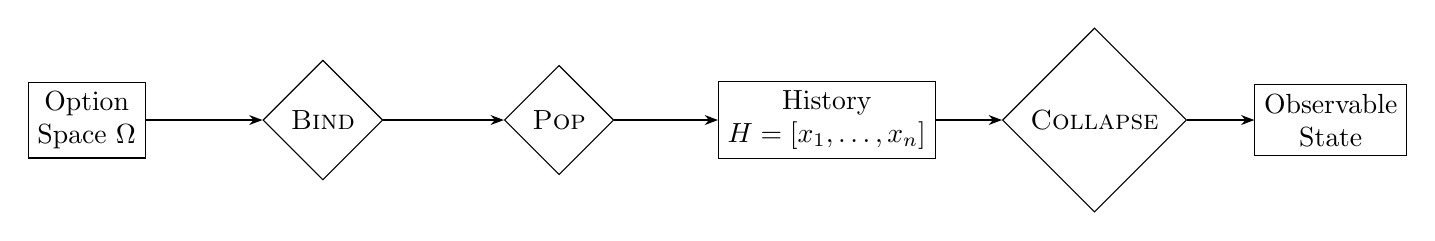
\begin{tikzpicture}[>=Stealth,node distance=2.6cm]
\node[draw,rectangle,align=center] (omega) {Option\\Space $\Option$};
\node[draw,diamond,right of=omega,xshift=0.4cm,align=center] (bind) {$\Bind$};
\node[draw,diamond,right of=bind,xshift=0.4cm,align=center] (pop) {$\Pop$};
\node[draw,rectangle,right of=pop,xshift=0.8cm,align=center] (hist) {History\\$H=\Seq{x_1,\dots,x_n}$};
\node[draw,diamond,right of=hist,xshift=0.8cm,align=center] (coll) {$\Collapse$};
\node[draw,rectangle,right of=coll,xshift=0.4cm,align=center] (state) {Observable\\State};
\draw[->] (omega) -- (bind);
\draw[->] (bind) -- (pop);
\draw[->] (pop) -- (hist);
\draw[->] (hist) -- (coll);
\draw[->] (coll) -- (state);
\end{tikzpicture}
\caption{The Spherepop semantic pipeline. Contextual restriction ($\Bind$) narrows the option space; irreversible commitment ($\Pop$) records selections in the append-only history; and observable state is reconstructed by applying $\Collapse$ to the resulting commitment sequence. In this formulation observable states are derived objects; the primary semantic structure is the append-only history of commitments.}
\end{figure}

% ============================================================
\begin{thebibliography}{99}
% ============================================================

\bibitem{maclane1998}
Saunders Mac Lane.
\textit{Categories for the Working Mathematician}.
2nd edition. Springer, 1998.

\bibitem{joyal1996}
Andr\'e Joyal, Ross Street, and Dominic Verity.
Traced monoidal categories.
\textit{Mathematical Proceedings of the Cambridge Philosophical Society},
119(3):447--468, 1996.

\bibitem{abramsky1994}
Samson Abramsky and Achim Jung.
Domain theory.
In \textit{Handbook of Logic in Computer Science}, Volume 3.
Oxford University Press, 1994.

\bibitem{winskel1995}
Glynn Winskel and Mogens Nielsen.
Models for concurrency.
In \textit{Handbook of Logic in Computer Science}, Volume 4.
Oxford University Press, 1995.

\bibitem{lamport1978}
Leslie Lamport.
Time, clocks, and the ordering of events in a distributed system.
\textit{Communications of the ACM}, 21(7):558--565, 1978.

\bibitem{fowler2005}
Martin Fowler.
Event sourcing.
\texttt{martinfowler.com}, 2005.

\bibitem{kleppmann2017}
Martin Kleppmann.
\textit{Designing Data-Intensive Applications}.
O'Reilly Media, 2017.

\bibitem{shapiro2011}
Marc Shapiro, Nuno Pregui\c{c}a, Carlos Baquero, and Marek Zawirski.
Conflict-free replicated data types.
In \textit{Stabilization, Safety, and Security of Distributed Systems (SSS)}, 2011.

\bibitem{chacon2014}
Scott Chacon and Ben Straub.
\textit{Pro Git}.
Apress, 2014.

\bibitem{brightwell1991}
Graham Brightwell and Rafael Sorkin.
Structure of causal sets.
\textit{Physical Review D}, 44(4):1027--1037, 1991.

\bibitem{hopcroft2006}
John Hopcroft, Rajeev Motwani, and Jeffrey Ullman.
\textit{Introduction to Automata Theory, Languages, and Computation}.
3rd edition. Pearson, 2006.

\end{thebibliography}

\end{document}
